% allgem. Dokumentenformat
\documentclass[a4paper,12pt,headsepline]{scrartcl}
%Variablen welche innerhalb der gesamten Arbeit zur Verfügung stehen sollen
\newcommand{\titleDocument}{Bachelor- / Masterarbeit}
\newcommand{\subjectDocument}{im Studiengang <Studiengang>}

% weitere Pakete
% Grafiken aus PNG Dateien einbinden
\usepackage{graphicx}

% deutsche Silbentrennung
%\usepackage[ngerman]{babel}

% Eurozeichen einbinden
\usepackage[right]{eurosym}

% Umlaute unter UTF8 nutzen
\usepackage[utf8]{inputenc}

% Zeichenencoding
\usepackage[T1]{fontenc}

\usepackage{lmodern}
\usepackage{fix-cm}

% floatende Bilder ermöglichen
%\usepackage{floatflt}

% mehrseitige Tabellen ermöglichen
\usepackage{longtable}

% Unterstützung für Schriftarten
%\newcommand{\changefont}[3]{ 
%\fontfamily{#1} \fontseries{#2} \fontshape{#3} \selectfont}

% Packet für Seitenrandabständex und Einstellung für Seitenränder
\usepackage{geometry}
\geometry{left=3.5cm, right=2cm, top=2.5cm, bottom=2cm}

% Paket für Boxen im Text
\usepackage{fancybox}

% bricht lange URLs "schoen" um
\usepackage[hyphens,obeyspaces,spaces]{url}

% Paket für Textfarben
\usepackage{color}

% Mathematische Symbole importieren
\usepackage{amssymb}

% auf jeder Seite eine Überschrift (alt, zentriert)
%\pagestyle{headings}

% erzeugt Inhaltsverzeichnis mit Querverweisen zu den Kapiteln (PDF Version)
\usepackage[bookmarksnumbered,pdftitle={\titleDocument},hyperfootnotes=false]{hyperref} 
%\hypersetup{colorlinks, citecolor=red, linkcolor=blue, urlcolor=black}
%\hypersetup{colorlinks, citecolor=black, linkcolor= black, urlcolor=black}

% neue Kopfzeilen mit fancypaket
\usepackage{fancyhdr} %Paket laden
\pagestyle{fancy} %eigener Seitenstil
\fancyhf{} %alle Kopf- und Fußzeilenfelder bereinigen
\fancyhead[L]{\nouppercase{\leftmark}} %Kopfzeile links
\fancyhead[C]{} %zentrierte Kopfzeile
\fancyhead[R]{\thepage} %Kopfzeile rechts
\renewcommand{\headrulewidth}{0.4pt} %obere Trennlinie
%\fancyfoot[C]{\thepage} %Seitennummer
%\renewcommand{\footrulewidth}{0.4pt} %untere Trennlinie

% für Tabellen
\usepackage{array}

% Runde Klammern für Zitate
%\usepackage[numbers,round]{natbib}

% Festlegung Art der Zitierung - Havardmethode: Abkuerzung Autor + Jahr
\bibliographystyle{alphadin}

% Schaltet den zusätzlichen Zwischenraum ab, den LaTeX normalerweise nach einem Satzzeichen einfügt.
\frenchspacing

% Paket für Zeilenabstand
\usepackage{setspace}

% für Bildbezeichner
\usepackage{capt-of}

% für Stichwortverzeichnis
\usepackage{makeidx}

% für Listings
\usepackage{listings}
\lstset{numbers=left, numberstyle=\tiny, numbersep=5pt, keywordstyle=\color{black}\bfseries, stringstyle=\ttfamily,showstringspaces=false,basicstyle=\footnotesize,captionpos=b}
\lstset{language=java}

% Indexerstellung
\makeindex

% Abkürzungsverzeichnis
\usepackage[german]{nomencl}
\let\abbrev\nomenclature

% Abkürzungsverzeichnis LiveTex Version
\renewcommand{\nomname}{Abkürzungsverzeichnis}
\setlength{\nomlabelwidth}{.25\hsize}
\renewcommand{\nomlabel}[1]{#1 \dotfill}
\setlength{\nomitemsep}{-\parsep}
\makenomenclature
%\makeglossary

% Abkürzungsverzeichnis TeTEX Version
% \usepackage[german]{nomencl}
% \makenomenclature
% %\makeglossary
% \renewcommand{\nomname}{Abkürzungsverzeichnis}
% \setlength{\nomlabelwidth}{.25\hsize}
% \renewcommand{\nomlabel}[1]{#1 \dotfill}
% \setlength{\nomitemsep}{-\parsep}

% Disable single lines at the start of a paragraph
\clubpenalty = 10000
% Disable single lines at the end of a paragraph
\widowpenalty = 10000
\displaywidowpenalty = 10000

\begin{document}
% hier werden die Trennvorschläge inkludiert
%hier müssen alle Wörter rein, welche Latex von sich auch nicht korrekt trennt bzw. bei denen man die genaue Trennung vorgeben möchte
\hyphenation{
Film-pro-du-zen-ten
Lux-em-burg
Soft-ware-bau-steins
zeit-in-ten-siv
}

%Schriftart Helvetica
%\changefont{phv}{m}{n}

% Leere Seite am Anfang
\newpage
\thispagestyle{empty} % erzeugt Seite ohne Kopf- / Fusszeile
\section*{ }

% Titelseite %
% das Papierformat zuerst
%\documentclass[a4paper, 11pt]{article}

% deutsche Silbentrennung
%\usepackage[ngerman]{babel}

% wegen deutschen Umlauten
%\usepackage[ansinew]{inputenc}

% hier beginnt das Dokument
%\begin{document}


\thispagestyle{empty}

% \begin{figure}[t]
%  \centering
%  
\includegraphics[width=0.4\textwidth]{abb/hd_logo_small_sw_16cm_rgb}
% \end{figure}

%\begin{figure}[t]
% \centering
% 
\includegraphics[width=0.3\textwidth]{abb/hd_logo_small_sw_16cm_rgb}
%~~~~~~~~~~
% 
\includegraphics[width=0.3\textwidth]{abb/ziti-logo_150}
%\end{figure}


\begin{verbatim}


\end{verbatim}

\begin{center}
\Large{Heidelberg University}\\
%\Large{- Campus <Name> -}\\
\end{center}


\begin{center}
\Large{Institute of Computer Engineering (ZITI)}
\end{center}
\begin{verbatim}




\end{verbatim}
\begin{center}
\doublespacing
\textbf{\LARGE{Univeral Verification Methodology Multi-Language}}\\
\medskip
\textbf{\large{Student Research Project}}\\
\singlespacing
\begin{verbatim}

\end{verbatim}
%\textbf{Master of Science}\\
%\textbf{Computer Engineering (Technische Informatik)}\\
%\textbf{MScTI}
\end{center}
\begin{verbatim}

\end{verbatim}
\begin{center}

\end{center}
%\begin{verbatim}

% \end{verbatim}
% \begin{center}
% \textbf{zur Erlangung des akademischen Grades \\ Bachelor / Master of Science}
% \end{center}
% \begin{verbatim}






%\end{verbatim}
\vfil

\begin{flushleft}
\begin{tabular}{llll}
%\textbf{Topic:} & & Universal Verification Methodology Multi-Language & \\
& & \\
\textbf{Author:} & & Sebastian Wittka BEng. email:
wittka\{at\}stud.uni-heidelberg.de&
\\
& & Student Number: 3239353 & \\
& & \\
\textbf{Version of:} & & \today &\\
& & \\
\textbf{Advisor:} & & Dr. Niels Burkhardt &\\
\end{tabular}
\end{flushleft}


% römische Numerierung
%\pagenumbering{arabic}

% 1.5 facher Zeilenabstand
\onehalfspacing

% Sperrvermerk
%\section*{Sperrvermerk}
\textcolor{red}{
Die vorliegende Arbeit beinhaltet interne und vertrauliche Informationen der Firma <Firmenname>.
Die Weitergabe des Inhalts der Arbeit im Gesamten oder in Teilen sowie das Anfertigen
von Kopien oder Abschriften - auch in digitaler Form - sind grundsätzlich untersagt.
Ausnahmen bedürfen der schriftlichen Genehmigung der Firma <Firmenname>.
}

% Einleitung / Abstract
\section*{Abstract}
One of the essential objectives of functional verification is to reuse verification code when moving from one verification level to a higher one. Therefore lower level components have to be integrated into a hierarchy with other components. This cannot be done without further ado, if the components are implemented in different verification languages. So fully operative code would have to be rewritten from scratch. This time consuming approach can be avoided by using the open source \emph{Universal Verification Methodology Multi-Language} package provided by Accellera. It allows the reuse of verification components of different languages to build a fully operative multi-languages testbench. This report shows how to use this package to reuse UVM-SystemVerilog components in UVM-\textit{e} ones and vice versa, especially how to build a multi-language testbench, configure it and establish communication between the components. Furthermore it is demonstrated how to execute sequences and sequence items of foreign components. Eventually it is evaluated, which parts of the package have to be improved to ensure building a multi-language testbench with less effort. Particularly implementing an integrated end of test synchronization as well as a less effortful method of reusing foreign sequences.

% einfacher Zeilenabstand
\singlespacing

% Eidesstattliche Erklärung
\addcontentsline{toc}{section}{Declaration of Authorship}
\section*{Eidesstattliche Erklärung}
\thispagestyle{empty}

\begin{verbatim}

\end{verbatim}

\begin{LARGE}Eidesstattliche Erklärung zur <-Arbeit>\end{LARGE}
\begin{verbatim}


\end{verbatim}
Ich versichere, die von mir vorgelegte Arbeit selbstständig verfasst zu haben. Alle Stellen, die wörtlich oder sinngemäß aus veröffentlichten oder nicht veröffentlichten Arbeiten anderer entnommen sind, habe ich als entnommen kenntlich gemacht. Sämtliche Quellen und Hilfsmittel, die ich für die Arbeit benutzt habe, sind angegeben. Die Arbeit hat mit gleichem Inhalt bzw. in wesentlichen Teilen noch keiner anderen Prüfungsbehörde vorgelegen.



\begin{displaymath}
% use packages: array
\begin{array}{ll}
Unterschrift:~~~~~~~~~~~~~~~~~~~~~~~~~~~~~~~~~~~~~~~~~~
& Ort, Datum:~~~~~~~~~~~~~~~~~~~~~~~~~~~~~~~~~~~~~~~~~~
\end{array}
\end{displaymath}


% Inhaltsverzeichnis anzeigen
\newpage
\tableofcontents

% das Abbildungsverzeichnis
%\newpage
% Abbildungsverzeichnis soll im Inhaltsverzeichnis auftauchen
\addcontentsline{toc}{section}{Abbildungsverzeichnis}
% Abbildungsverzeichnis endgueltig anzeigen
\listoffigures

% das Tabellenverzeichnis
%\newpage
% Abbildungsverzeichnis soll im Inhaltsverzeichnis auftauchen
\addcontentsline{toc}{section}{Tabellenverzeichnis}
% \fancyhead[L]{Abbildungsverzeichnis / Abkürzungsverzeichnis} %Kopfzeile links
% Abbildungsverzeichnis endgueltig anzeigen
\listoftables

%% WORKAROUND für Listings
%\makeatletter% --> De-TeX-FAQ
%\renewcommand*{\lstlistoflistings}{%
%  \begingroup
%    \if@twocolumn
%      \@restonecoltrue\onecolumn
%    \else
%      \@restonecolfalse
%    \fi
%    \lol@heading
%    \setlength{\parskip}{\z@}%
%    \setlength{\parindent}{\z@}%
%    \setlength{\parfillskip}{\z@ \@plus 1fil}%
%    \@starttoc{lol}%
%    \if@restonecol\twocolumn\fi
%  \endgroup
%}
%\makeatother% --> \makeatletter
% das Listingverzeichnis
%\newpage
% Listingverzeichnis soll im Inhaltsverzeichnis auftauchen
\addcontentsline{toc}{section}{Listingverzeichnis}
\fancyhead[L]{Abbildungs- / Tabellen- / Listingverzeichnis} %Kopfzeile links
\renewcommand{\lstlistlistingname}{Listingverzeichnis}
\lstlistoflistings
%%%%

% das Abkürzungsverzeichnis
%\newpage
% Abkürzungsverzeichnis soll im Inhaltsverzeichnis auftauchen
\addcontentsline{toc}{section}{Abkürzungsverzeichnis}
% das Abkürzungsverzeichnis entgültige Ausgeben
\fancyhead[L]{Abkürzungsverzeichnis} %Kopfzeile links
\nomenclature{UGC}{User Generated Content}
\nomenclature{CSS}{Cascading Style Sheets}
\nomenclature{JS}{JavaScript}
\nomenclature{SQL}{Structured Query Language}
\nomenclature{GPL}{GNU General Public License}
\nomenclature{GNU}{GNU is not Unix}
\nomenclature{LGPL}{GNU Lesser General Public License}
\nomenclature{XMPP}{Extensible Messaging and Presence Protocol}
\nomenclature{IM}{Instant Message}
\nomenclature{CMS}{Content Management System}
\nomenclature{RSS}{Really Simple Syndication}
\nomenclature{JSON}{JavaScript Object Notation}
\nomenclature{HTML}{Hypertext Markup Language}
\nomenclature{TDD}{Test-driven development}
\nomenclature{GUI}{Graphical User Interface}
\nomenclature{KPI}{Key Performance Indicator}
\nomenclature{WWW}{World Wide Web}
\nomenclature{OCR}{Optical Character Recognition}
\nomenclature{ERM}{Entity Relationship Modell}

\printnomenclature

% Definiert Stegbreite bei zweispaltigem Layout
\setlength{\columnsep}{25pt}

%%%%%%% EINLEITUNG %%%%%%%%%%%%
%\twocolumn
\newpage
\fancyhead[L]{\nouppercase{\leftmark}} %Kopfzeile links

% 1,5 facher Zeilenabstand
\onehalfspacing

% einzelne Kapitel
\section{Introduction}\label{introduction}
When designing an \emph{application-specific integrated circuit (ASIC)} it is
necessary to divide it into logical units called modules, so its complexity is
reduced to multiple manageable problems. Considering this it is obvious to use the same
strategy when designing the verification environment of this chip. A commonly
used approach to get such a hierarchical test bench is to use the \emph{Univeral
Verification Methodology (UVM)} to divide the test bench into reusable
subcomponents. The resulting units are called \emph{Universal Verification
Components (UVCs)}. Such test benches are written in special verification
languages like \emph{Systemverilog}, \emph{e} or \emph{SystemC}.\\
Because the structure of an UVC supports reusability, it is typical that an UVC
is utilized again when its corresponding module is reused in another design. Now
it can occur that the test bench for the new design uses another verification
language than the reused UVC. In this case the previous created UVC cannot be
used and must be rewritten in the verification language of the new test bench.
This means that additional time is needed to implement and test the UVC, which
actually already existed, just in another verification language. Therefore it
would be preferable to build a test bench consisting of UVCs regardless of the
verification language they are implemented in.\\
This is the idea behind  \emph{Universal Verification Language
Multi-Language (UVM-ML)}. It is an open source solution to integrate
verification components written in different languages into a single
environment and its features are introduced in this paper.






\section{Summary of the Universal Verification Methodology}\label{uvm}
- ca. 3 pages
\\
- 1/2 page\\
-what is UVM?\\
-why should you use UVM?\\
-different types of UVCs (interface, module)\\
\subsection{Interface UVC} (1 page)\\
- environment, slave/master agent, bfm, sequence driver, sequences, monitor\\
- active/passive\\
\subsection{Module UVC} (1 page)\\
- environment, monitor, scoreboard, reference model\\
\subsection{Data Communication between Components} (1/2 page)\\
- TLM-Ports\\


\section{Universal Verification Methodology Multi-Language}\label{uvm_ml}
\todo[inline]{all emph are set for names}
\todo[inline]{textit for e}
\todo[inline]{nice layout}
\todo[inline]{do not mix framework and verification language}
\todo[inline]{abbreviations introduced only once}
Verification projects consist of ready to use verification components, which are joined in a testbench. These components
are often implemented in different verification languages like \emph{SystemVerilog}, \textit{e} or \emph{SystemC}. For
example, when verification projects are normally implemented in \textit{e}, but some components are intellectual
property and provide UVCs implemented in \emph{SystemVerilog}. This leads to the demand of re-implementing fully
operative code just for switching the verification language.\\
Such a time consuming approach to this problem can be avoided by using the \emph{Universal Verification Methodology
Multi-Language} (UVM-ML) package developed in cooperation of Advanced Micro Devices, Inc. (AMD) and Cadence Design
Systems, Inc. It is based on the \emph{Universal Verification Methodology} and extends it multi-language
functionalities. These enable the joined use of components implemented in different verification languages to build a
single testbench with minimal changes of the reused components.\\
This paper focuses on the two verification languages \emph{SystemVerilog} and \textit{e} both using the \emph{Universal
Verification Methodology} to show the capabilities provided by UVM-ML. The simulator used for this is the
\emph{Incisive Enterprise Simulator} developed by \emph{Cadence Design Systems, Inc.}\\
The key concepts, which provide these capabilities are described in the following section. After that it is shown how to
integrate multi-language functionalities into \emph{Incisive Enterprise Simulator}. Followed by the illustration on how
to use it to create an multi-language environment, configure its sub-components and enable data communication between
components. Finally it is declared how to start a test in this environment.

\subsection{Key concepts of UVM-ML}

The primary goal of the UVM-ML open architecture solution is to expand the UVM scope from a single language to multiple
languages. Thereby it is independent of the simulator used and can be extended to support additional verification
languages. The main elements used in the multi-language library are the language frameworks, the framework adapters and
the multi-language backplane.
\begin{itemize}
  \item\textbf{Framework}\\
  Frameworks are the combination of the language and the methodology used to develop verification components. Some
  examples are \emph{UVM-SystemVerilog}, \emph{UVM-SystemC} and \emph{UVM-\textit{e}}.
  \item\textbf{Backplane}\\
  The backplane is the central component of the multi-language architecture and connects the frameworks in a star
  topology.
  It is only internal to UVM-ML and cannot be accessed directly by the user code.
  \item\textbf{Adapter}\\
  Adapters build the bridge between frameworks and the backplane. They provide all multi-language functionalities for
  the frameworks so they are unaware of the backplane.
\end{itemize}

\begin{figure}[htb]
 \centering
 %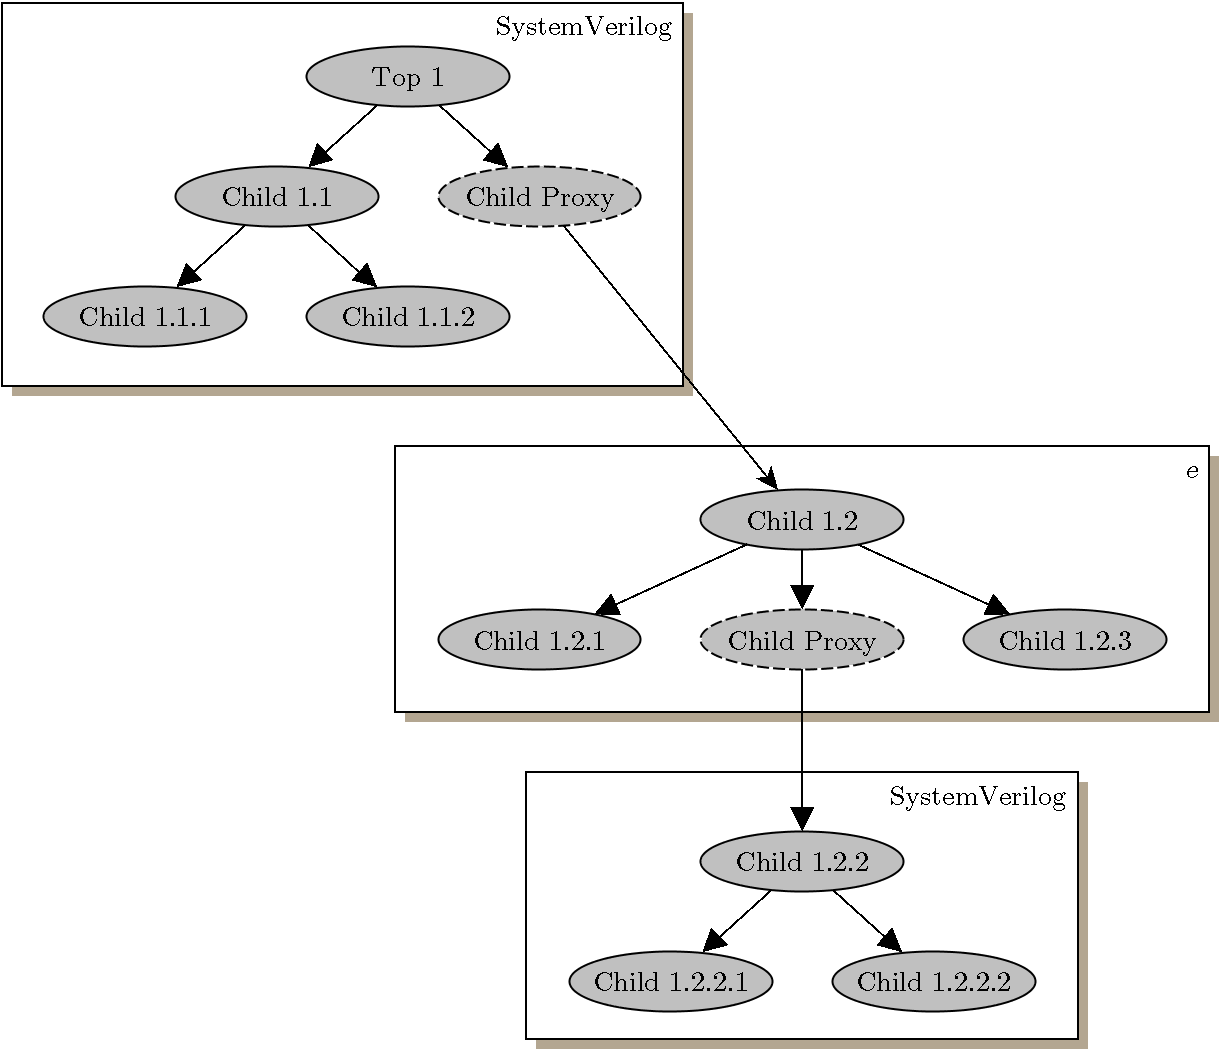
\includegraphics[width=1.0\textwidth,angle=0]{abb/UVM_ML_unified}
 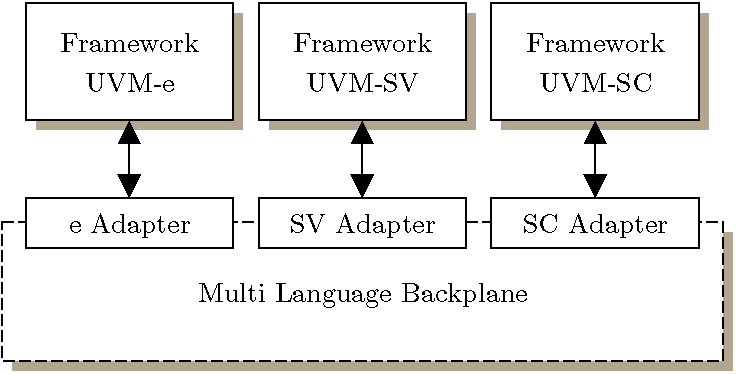
\includegraphics[scale=0.3]{abb/UVM_ML_architecture}
 \caption{UVM-ML architecture}
\label{fig:UVM_ML_architecture}
\end{figure}

The basic structure of the multi-language architecture is displayed in figure~\ref{fig:UVM_ML_architecture}. Each
framework accesses the backplane exclusively through its corresponding adapter. There are only the three adapters shown,
which are provided by the UVM-ML package, but it can be extended to support other frameworks as well.

\subsection{Integrate Multi-Language Functionality into Incisive Enterprise
Simulator}
At the current state of work multi-language support can be integrated into Cadence Incisive Enterprise Simulator (IES)
via an open source package provided by Accellera Systems Initiative and developed jointly by AMD and Cadence Design
Systems. This package is called \emph{UVM-ML Open Architecture} and is provided as download on the Accellera website.
For this paper version 1.5.1 of the package was used. After downloading and extracting it can be
installed via the provided install script called \emph{install\_ies.csh} and the following steps using \emph{C shell}:

\medskip
\lstset{language={}, numbers=none, escapechar=|}
\begin{lstlisting}
% setenv UVM_ML_HOME <install_dir>
% set path= (<path_to_irun> $path)
% source $UVM_ML_HOME/ml/install_ies.csh [--64bit] [--no-osci]
\end{lstlisting} 
\medskip 

Using \emph{Bourne shell} the corresponding commands are:

\medskip
\lstset{language={}, numbers=none, escapechar=|}
\begin{lstlisting}
% export UVM_ML_HOME=<install_dir>
% export PATH=<path_to_irun>:$PATH
% csh -c "source $UVM_ML_HOME/ml/install_ies.csh [--64bit] [--no-osci]"
\end{lstlisting} 
\medskip 

Due to some problems with the installation on \emph{Ubuntu} it is recommended to use an alternative distribution like
\emph{CentOS}. The environment variable \emph{UVM\_ML\_HOME} needs to point to the root directory of the UVM-ML
package, which is \emph{UVM\_ML-1.5.1} for version 1.5.1. When already using IES, the standard setup script can be used
instead of manually setting the path environment variable to the \emph{irun} installation. While sourcing
\lstinline$install_ies.csh$ additional options can be used to control it. To install the environment on a 64 bit machine
instead of an 32 bit one use \lstinline$--64bit$. If only the adapters for UVM-SystemVerilog, UVM-SystemC and
UVM-\textit{e} are required, UVM-ML can be build without the ASI-SystemC adapter via \lstinline$--no_osci$.\\
After this intallation UVM-ML enables the creation of multi-language environments as well as running tests, which is
discussed in the following sections.

\subsection{Creating a Multi-Language Environment}
A verification environment typically consists of a system UVC containing
multiple subsystem UVCs, interface UVCs or module UVCs. These are composed in a
hierarchical way. With UVM-ML an environment can be constructed with components,
which are implemented in different frameworks. For example it could be composed
of an interface UVC implemented in UVM-SV and a module UVC in
UVM-\textit{e}. \\
When planing to create such a multi-language environment, there
are two possible approaches supported by UVM-ML to achieve this goal. Firstly an
\emph{unified hierarchy} can be created or alternatively an \emph{side-by-side}
environment. In an unified hierarchy a child component implemented in one
verification language is instantiated from a parent component in another
verification language. In contrast, when creating a side-by-side architecture,
the environment contains multiple tops.

\subsubsection{Creating an \emph{Unified Hierarchy} Environment}
To implement an \emph{unified hierarchy} each component which instantiates a
component of another framework needs to create and connect a proxy to
this component (this can be seen in figure~\ref{fig:UVM_ML_unified}). Then the
backplane applies operations which are performed on the proxy to the
corresponding component in the other verification language. This gives the
opportunity to use some of UVM-ML's benefits. It is possible to use a predefined
phasing in this environment, where phases like build, connect or run are
performed depth-first to ensure that dependencies between the components of
different frameworks are resolved in the right way. Also sub-components can be
configured which increases the reusability of the environment, because when the
environment is included in some other environment, only the top component needs
to be configured and all sub-components are configured automatically. Because of
this it is recommended to implement such an environment.\\
Following it is described how to create a \emph{unified hierarchy} which
instantiates a SystemVerilog component within an \textit{e} unit and vice versa.

\begin{figure}[htb]
 \centering
 %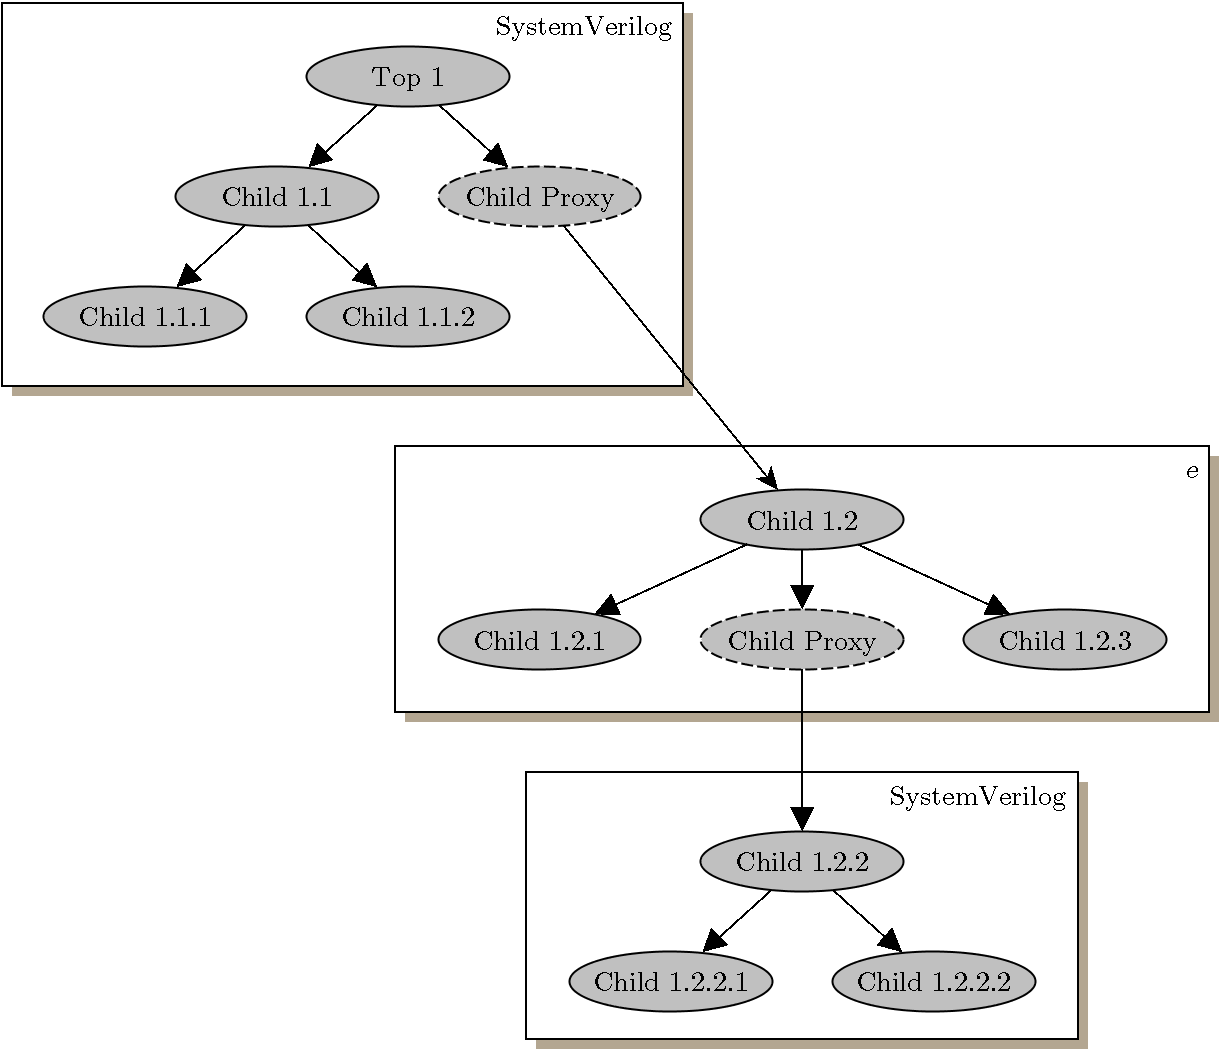
\includegraphics[width=1.0\textwidth,angle=0]{abb/UVM_ML_unified}
 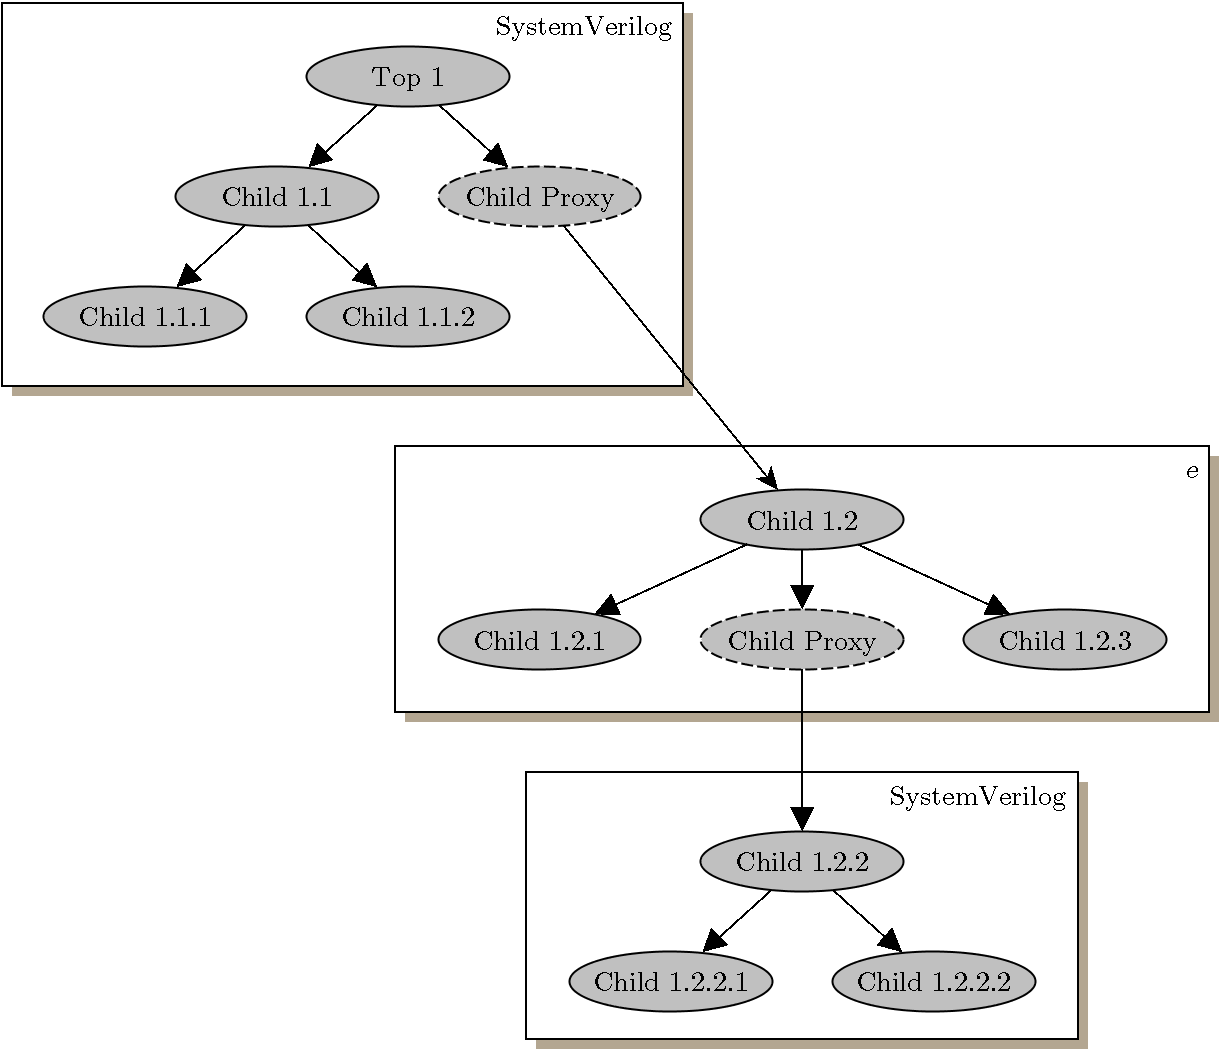
\includegraphics[scale=0.3]{abb/UVM_ML_unified}
 \caption{Structure of an \emph{unified hierarchy} environment}
\label{fig:UVM_ML_unified}
\end{figure}

\paragraph{Instantiating a SystemVerilog Component within an \textit{e} Unit}
\label{sv_inside_e}
When instantiating a SystemVerilog component within an \textit{e} unit,
it is necessary to instantiate a proxy unit inside the \textit{e} unit. After that the
proxy unit and the SystemVerilog component need to be connected. \\
An example for the code of the extended SystemVerilog component can be seen in
\emph{example~\ref{lst:SV_unified_sub}}.
It is recommended to extend the SystemVerilog component
(line~\ref{line_extend_component}) which will
be reused and then put all multi-language functionalities inside this new
component to ensure that the original component can still be used in
non-multi-language environments. The extended one needs to include the UVM
package (line~\ref{line_uvm_package}/\ref{line_uvm_macros}) as well as the adapter
package for SystemVerilog (line~\ref{line_uvm_ml_package}).
After that all additional multi-language functionalities can be put inside the
class like configuring this sub-component (see section~\ref{ml_config}) or data
communication via TLM ports (see section~\ref{ml_tlm}).
\medskip
\lstset{language={SystemVerilog}, numbers=left, escapechar=|}
\begin{lstlisting}[frame=htrbl, caption={SystemVerilog: extended component}, label={lst:SV_unified_sub}]
import uvm_pkg::*;					|\label{line_uvm_package}|
`include "uvm_macros.svh"			|\label{line_uvm_macros}|
import uvm_ml::*;					|\label{line_uvm_ml_package}|

class ml_ubus_env extends ubus_env;			|\label{line_extend_component}|
  `uvm_component_utils(ml_ubus_env)
  function void build_phase(uvm_phase phase);
    // Additional multi-language functionalities
  endfunction : build_phase
endclass : ml_ubus_env
\end{lstlisting}
\medskip
Corresponding to the extensions in the SystemVerilog component the \textit{e}
unit needs to include an proxy unit for it (see \emph{example~\ref{lst:e_unified_top}}).
This can be done by instantiating an unit of type
\lstinline$child_component_proxy$ (line~\ref{line_uvm_ml_e_proxy}) which is a
predefined data type in \textit{e}.
Through constraining the proxy unit's \lstinline$type_name$ field
(line~\ref{line_uvm_ml_e_proxy_keep}) the
SystemVerilog component is integrated into the hierarchy. Thereby the string
needs to be composed of \lstinline$target_frmw_indicator:component_type_name$, where
\lstinline$target_frmw_indicator$ (case-insensitive) identifies the framework
of the instantiated foreign child component and can be \lstinline$SV$ for
UVM-SystemVerilog, \lstinline$e$ for UVM-\textit{e} or \lstinline$SC$ for UVM-SystemC and
\lstinline$component_type_name$ is the type of the instantiated component.
\medskip
\lstset{language=e, numbers=left, escapechar=|}
\begin{lstlisting}[frame=htrbl, caption={\textit{e}: instantiating the SystemVerilog component in the \textit{e} unit},
label={lst:e_unified_top}]
unit ubus_env {
  uvc_top: child_component_proxy is instance;	|\label{line_uvm_ml_e_proxy}|
    keep uvc_top.type_name =|\,\,|= "SV:ml_ubus_env";|\label{line_uvm_ml_e_proxy_keep}| 
};
\end{lstlisting}

\paragraph{Instantiating an \textit{e} Unit Within a SystemVerilog Component}
When reusing an \textit{e} unit inside of an SystemVerilog component it is
necessary to integrate an proxy for the e unit within the SystemVerilog
component and then connect both.\\
As shown in \emph{example~\ref{lst:SV_unified_top}} this proxy component is created by
declaring an component of type \lstinline$uvm_component$ inside the parent
component (line~\ref{line_sv_declare_proxy}). In the \lstinline$build_phase$ this proxy component is
instantiated via calling \lstinline$uvm_ml_create_component$ (line~\ref{line_sv_create_proxy}) with the following
syntax:
\medskip
\lstset{language={}, numbers=none, escapechar=|}
\begin{lstlisting}
function uvm_ml::child_component_proxy uvm_ml_create_component(
  string target_frmw_indicator,
  string component_type_name,
  string instance_name,
  uvm_component parent=null)
\end{lstlisting} 
\medskip
Where \lstinline$target_frmw_indicator$ indicates the framework adapter of the
foreign component (see section~\ref{sv_inside_e}),
\lstinline$component_type_name$ is the type of the foreign component according
to its declaration inside its framework, \lstinline$instance_name$ is the name
of the instance of the component proxy and \lstinline$parent$ is the handle of
the parent instance (\lstinline$this$ indicates the current component).\\
Because multi-language functionality is already integrated in UVM-\textit{e}, the child unit does not need any changes
to support the creation of an \emph{unified hierarchy} environment.
\medskip
\lstset{language=SystemVerilog, numbers = left, escapechar=|, breaklines=true}
\begin{lstlisting}[frame=htrbl, caption={SystemVerilog: instantiating an e unit}, label={lst:SV_unified_top}]
class testbench extends uvm_env;
  uvm_component xbus_uvc;|\label{line_sv_declare_proxy}|
  `uvm_component_utils(testbench)

  function void build_phase(uvm_phase phase);
    super.build_phase(phase);
    xbus_uvc = uvm_ml_create_component("e", "xbus_env_u", "xbus_uvc", this); |\label{line_sv_create_proxy}|
  endfunction
endclass : testbench
\end{lstlisting}

\subsubsection{Creating a \emph{Side-by-Side} Environment}

When there is no need for creating an \emph{unified hierarchy} environment, UVM-ML supports also the ability to build an
environment with multiple tops as displayed in figure~\ref{fig:UVM_ML_side_by_side}. Here each tree inside of an
framework has its root instantiated as top component. This architecture is called \emph{side-by-side} and best
applicable when there is only limited synchronization required between the components of different frameworks. This is
indicated by the limitations of the architecture. It is not possible to use multi-language configuration as described in
section~\ref{ml_config}. Additionally the behavior of the phase execution is limited. Here each phase is first executed
completely on one tree before moving on to the next one. 

\begin{figure}[htb]
 \centering
 %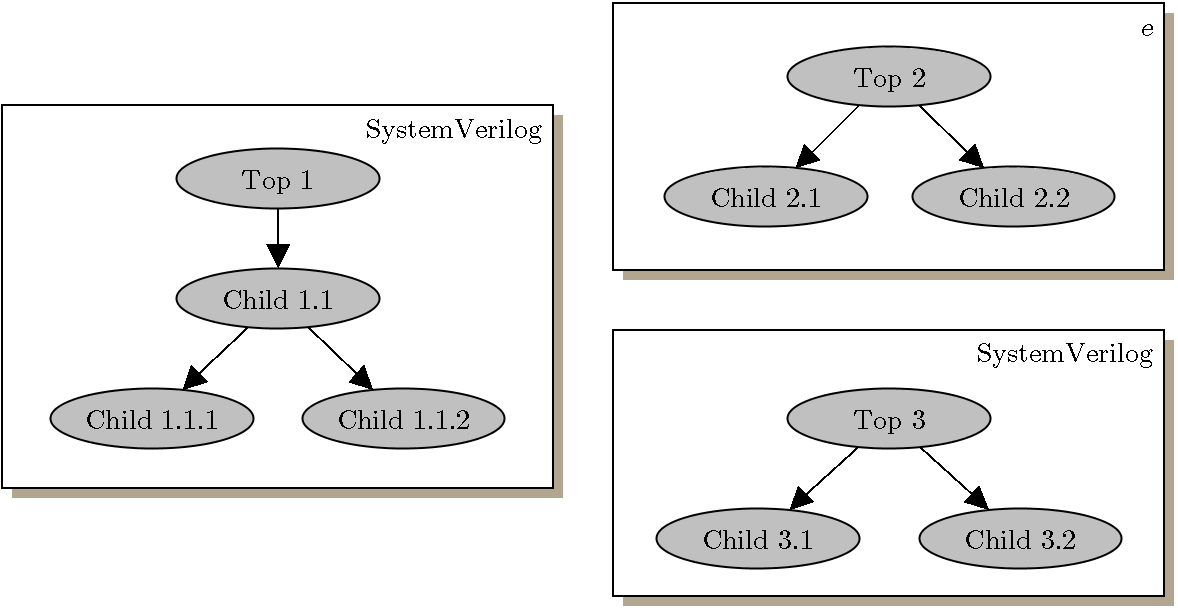
\includegraphics[width=1.0\textwidth,angle=0]{abb/UVM_ML_side_by_side}
 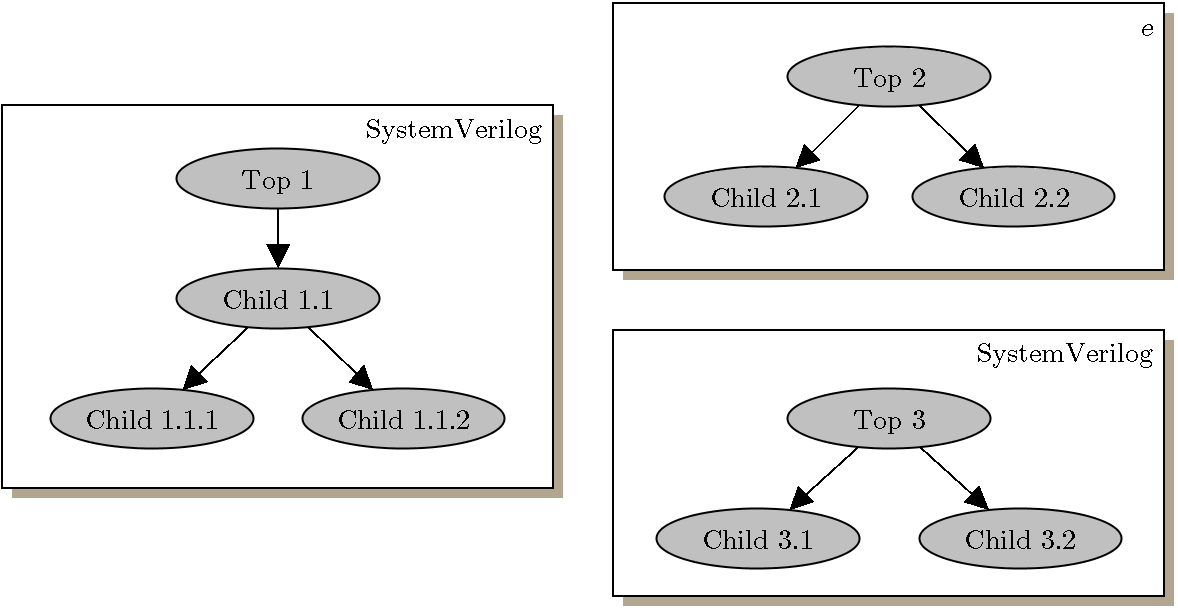
\includegraphics[scale=0.3]{abb/UVM_ML_side_by_side}
 \caption{Structure of an \emph{side-by-side} environment}
\label{fig:UVM_ML_side_by_side}
\end{figure}

\subsection{Mapping Data Items Across Frameworks }\label{type_mapping}
UVM-ML provides two options for data transfer between components of foreign frameworks. Firstly the configuration
database (see section~\ref{ml_config}), which gives tha ability to customize the structure of the multi-language
environment and secondly TLM communication for ongoing transfer of transactions between foreign components.\\
Both of them require, that the types of the transfered transactions match in both frameworks as well as the
serialization and de-serialization needs to match to ensure data consistence for both communication partners.

\subsubsection{Type Mapping}
Type mapping in an multi-language environment means, that a user defined type definition, like a struct or class, in
one framework is mapped to a corresponding type definition in another foreign framework. So the multi-language
backplane needs to know, which type definitions shall be mapped onto each other. By default this is implicitly done by
looking for equal type names.\\
If type names differ, but the type descriptions should be mapped onto each other, the mapping can be done expicitly.
For this purpose both, the SystemVerilog multi-language adapter as well as \textit{e} provide a function respectively
statement, which are shown below. Thereby \lstinline$frmw_indicator$ describes the framework, in wich the type is
declared (\lstinline$sv$ for UVM-SystemVerilog, \lstinline$e$ for UVM-\textit{e}) and \lstinline$type_name$ is the name
of the type within its framework.
\begin{itemize}
  \item{UVM-SystemVerilog}
\lstset{language={}, numbers=none, escapechar=|}
\begin{lstlisting}
set_type_match("frmw_indicator:type_name", "frmw_indicator:type_name");
\end{lstlisting} 
  \item{UVM-\textit{e}}
\lstset{language={}, numbers=none, escapechar=|}
\begin{lstlisting}
uvm_ml_type_match "frmw_indicator:type_name" "frmw_indicator:type_name"
\end{lstlisting} 
\end{itemize}

An example for both multi-language adapters mapping functionality is shown in example~\ref{lst:SV_type_mapping}
respectively example~\ref{lst:e_type_mapping}, where the struct \lstinline$e_packet$ is mapped onto the class
\lstinline$sv_packet$. Take into account, that the explicit type mapping only needs to occur in one component, either in
the \emph{SystemVerilog} component (example~\ref{lst:SV_type_mapping}, line~\ref{line_sv_mapping}) or the
\textit{e} unit (example~\ref{lst:e_type_mapping}, line~\ref{line_e_mapping}).

\lstset{language=SystemVerilog, numbers = left, escapechar=|, breaklines=true}
\begin{lstlisting}[frame=htrbl, caption={SystemVerilog: mapping \lstinline$sv_packet$ onto \lstinline$e_packet$},
label={lst:SV_type_mapping}]
class sv_packet extends uvm_transaction;
  int data;
  
  `uvm_object_utils_begin(sv_packet)
  `uvm_field_int(data, UVM_ALL_ON)|\label{line_sv_physical}|
  `uvm_object_utils_end
endclass : sv_packet

class testbench extends uvm_env;
  function void build_phase(uvm_phase phase);
    super.build_phase(phase);
    void'(set_type_match("e:e_packet", "sv:sv_packet"));|\label{line_sv_mapping}|
  endfunction : build_phase
endclass : testbench
\end{lstlisting}

\lstset{language=e, numbers = left, escapechar=|, breaklines=true}
\begin{lstlisting}[frame=htrbl, caption={\textit{e}: mapping \lstinline$sv_packet$ onto \lstinline$e_packet$},
label={lst:e_type_mapping}]
struct e_packet like any_struct {
  %data : int;|\label{line_e_physical}|
};

uvm_ml_type_match "e:e_packet" "sv:sv_packet"|\label{line_e_mapping}|
\end{lstlisting}

\subsubsection{Serialization and De-Serialization}
When transactions are transmitted across multiple frameworks, their representation inside of one framework cannot
directly be transferred into a foreign framework. Even if they are composed of the same fields, the internal
representation differ between frameworks. Therefore transactions are firstly serialized into an universal bitstream,
then this bitstream is transmitted to the foreign framework and finally de-serialized to extract the transaction from
it.\\
UVM-SystemVerilog as well as UVM-\textit{e} support default serialization and de-serialization. To use this
functionalities,  the order and type of fields in the transactions must match between the declarations. Only fields,
which are marked with a leading \lstinline$%$ are used for serialization and de-serialization in UVM-\textit{e} (see
example~\ref{lst:e_type_mapping}, line~\ref{line_e_physical} ) and other fields inside the struct are ignored. The same
occurs in UVM-SystemVerilog for fields, if the \lstinline$`uvm_field_*$ macro is defined for them with the flag for
packing/unpacking set within the macro (see example~\ref{lst:SV_type_mapping}, line~\ref{line_sv_physical}).\\
If the default serialization and de-serialization cannot be applied to an transaction, manual ones can be created by
implementing \lstinline$do_pack()$ as well as \lstinline$do_unpack()$ for UVM-SystemVerilog transactions and
\lstinline$pack()$ as well as \lstinline$unpack$ for UVM-\textit{e}, but this is not further discussed in this paper. 
\subsection{Configuring a Multi-Language Environment} \label{ml_config}

After building a multi-language environment it is often necessary to perform additional configurations before starting a
test. For example, setting an agent as passive respectively active or the number of resources available. In an
environment with an \emph{unified hierarchy} such configurations can be propagated from one framework tree
to all sub-trees in other frameworks. This is achieved by using the native UVM configuration constructs of each
framework, which are listed below:
\begin{itemize}
\item{UVM-SystemVerilog:}
%\medskip
\lstset{language={}, numbers=none, escapechar=|}
\begin{lstlisting}
uvm_config_db#(T)::set()
uvm_config_db#(T)::get()
\end{lstlisting} 
%\medskip

\item{UVM-\textit{e}}
%\medskip
\lstset{language={}, numbers=none, escapechar=|}
\begin{lstlisting}
keep uvm_config_set()
keep uvm_config_get()
\end{lstlisting} 
%\medskip
\end{itemize}

Each framework maintains its own configuration database. These are synchronized automatically via the multi-language
backplane when a configuration is set. Thereby for getting the configuration information each framework just needs to
access its local database, which hides the multi-language functionality from each framework.

\subsubsection{\textit{e} Units Configuring \emph{SystemVerilog} Components}\label{e_config_sv}

When configuring \emph{SystemVerilog} components via \textit{e} units it is necessary to distinguish two cases. Firstly
configuring it via primitive data types, where the data can directly be registered and obtained and secondly using
configuration objects, which requires to obtain the object using its base class followed by a cast to its proper data
type.\\
Since UVM-ML version~1.4.4 the generic UVM-SystemVerilog syntax using \lstinline$uvm_config_db#(T)$ is supported, which
provides a more convenient option to configure user defined data types. 

\paragraph{Configuring \emph{SystemVerilog} Components using Primitive Data Types}\label{config_sv_primitive}

When data is passed from an \textit{e} unit to a \emph{SystemVerilog} component,
the \textit{e} unit needs to constrain \lstinline$uvm_config_set()$ as shown in \emph{example~\ref{lst:e_set_int}}
line~\ref{line_e_set_int}. In this example the value \lstinline$16'h7fff$ is assigned to the variable
\lstinline$slave0_max$ in all components, which contain the letters \lstinline$ubus_env$ in their full path.

\lstset{language=e, numbers = left, escapechar=|, breaklines=true}
\begin{lstlisting}[frame=htrbl, caption={\textit{e}: register an integer in configuration database},
label={lst:e_set_int}]
extend testbench {
    keep uvm_config_set("*ubus_env*", "slave0_max", 16'h7fff);|\label{line_e_set_int}|
};
\end{lstlisting}

After the configuration is set in the database by the \textit{e} unit, the \emph{SystemVerilog} component needs to get
the value from its database. When it has an primitive data type like an integer as in \emph{example~\ref{lst:SV_get_int}},
the corresponding \lstinline$uvm_config_*::get()$ method should be used as shown in line~\ref{line_sv_get_int}. Here the
value of \lstinline$slave0_max$ registered for this component in the database is assigned to the variable with the same
name, \lstinline$slave0_max$.\\
When the field was specified with the corresponding \lstinline$uvm_field_*$ macro, calling
\lstinline$uvm_config_*::get()$ is not required. Its value is automatically retrieved from the configuration database.

\lstset{language=SystemVerilog, numbers = left, escapechar=|, breaklines=true}
\begin{lstlisting}[frame=htrbl, caption={SystemVerilog: getting an integer from configuration database},
label={lst:SV_get_int}]
class ml_ubus_env extends ubus_env;
  int slave0_max;|\label{line_sv_declare_int}|
  function void end_of_elaboration_phase(uvm_phase phase);
    void'(uvm_config_int::get(this, "", "slave0_max", slave0_max));|\label{line_sv_get_int}|
  endfunction : end_of_elaboration_phase
endclass
\end{lstlisting}

\paragraph{Configuring \emph{SystemVerilog} Components using Objects}\label{e_config_sv_object}

When using configuration objects instead of primitive data types, the \textit{e} unit can access its configuration
database the same way as with an primitive data type as shown in \emph{example~\ref{lst:e_set_object}}. In this example
an object of type \lstinline$data$ is created (line~\ref{line_e_declare_object}) and then registered in the
configuration database (line~\ref{line_e_set_object}) the same way as for primitive data types
(section~\ref{config_sv_primitive}).

\lstset{language=e, numbers = left, escapechar=|, breaklines=true}
\begin{lstlisting}[frame=htrbl, caption={e: register an object in configuration database}, label={lst:e_set_object}]
struct data {
  % addr    : int;
  % trailer : int;
  % txt     : string;
};

unit u {
  my_sv_child: child_component_proxy is instance;
    keep my_sv_child.type_name == "SV:test";
  
  d : data;|\label{line_e_declare_object}|
    keep d.addr    == 10;
    keep d.trailer == 20;
    keep d.txt     == "config object msg";

  keep uvm_config_set("my_sv_child","conf_data",d);|\label{line_e_set_object}|
};
\end{lstlisting}
The difference between configuring a SystemVerilog component using a primitive data type compared to an object
is displayed in \emph{example~\ref{lst:SV_get_object}}. Additionally to the declaration of the object in
line~\ref{line_sv_declare_object} another one of type \lstinline$uvm_object$ is required
(line~\ref{line_sv_declare_data}). Configuration objects need to be derived from this base type as shown in
line~\ref{line_sv_class_object} (\lstinline$uvm_transaction$ inherits from \lstinline$uvm_object$).\\
When the field of type \lstinline$uvm_object$ was specified with the \lstinline$uvm_field_object$ macro, calling
\lstinline$uvm_config_object::get()$ is not required. Its value is automatically retrieved from the configuration
database and can then be casted directly to the proper data type.\\
As mentioned previously, the generic syntax using \lstinline$uvm_config_db#(T)$ can be used to obtain configuration
objects as an alternative to \lstinline$uvm_config_object$.
The benefit of this approach is, that an additional cast after getting the object is not required as shown in
line~\ref{line_sv_get_user_object}. The object with the user defined type \lstinline$data$ is directly obtained from
the database, so line \ref{line_sv_declare_object}, \ref{line_sv_get_object} and \ref{line_sv_cast_object} are replaced
by this single line of code.

\lstset{language=SystemVerilog, numbers = left, escapechar=|, breaklines=true}
\begin{lstlisting}[frame=htrbl, caption={SystemVerilog: getting a configuration object}, label={lst:SV_get_object}]
class data extends uvm_transaction;|\label{line_sv_class_object}|
  int addr;
  int trailer;
  string txt;
  
  `uvm_object_utils_begin(data)
    `uvm_field_int(   addr,    UVM_ALL_ON)
    `uvm_field_int(   trailer, UVM_ALL_ON)
    `uvm_field_string(txt,     UVM_ALL_ON)
  `uvm_object_utils_end
endclass

class test extends uvm_env;
  uvm_object tmp_obj;|\label{line_sv_declare_object}|
  data conf_data;|\label{line_sv_declare_data}|
  
  function void build_phase(uvm_phase phase);
    super.build_phase(phase);
    void'(uvm_config_object::get(this,"","conf_data", tmp_obj));|\label{line_sv_get_object}|
    assert($cast(conf_data,tmp_obj)!=0);|\label{line_sv_cast_object}|
    //-- alternativly uvm_config_db can be used
    //void'(uvm_config_db#(data)::get(this,"","conf_data",conf_data));|\label{line_sv_get_user_object}|
  endfunction
endclass
\end{lstlisting}
It is important that the declarations of the configuration object in both verification languages are mapped to each
other. This includes the number and order of variables as well as the name of the type definition. For more information
on type mapping see section~\ref{type_mapping}.

\subsubsection{SystemVerilog Components Configuring \textit{e} Units}
Similar to section~\ref{e_config_sv} \emph{SystemVerilog} components can configure \textit{e} units via the
configuration database. The syntax remains the same, just the part of getting respectively setting is switched for both
frameworks. The field that should be configured has to be registered in the database from the \emph{SystemVerilog}
component prior to creating the sub-component. Then the \textit{e} unit needs to be constrained using
\lstinline$uvm_config_get()$ to receive the value from the configuration database.

\paragraph{Configuring \textit{e} units using Primitive Data Types}
When configuring an \textit{e} unit via a \emph{SystemVerilog} component, the component needs to register the value in
the configuration database by calling \lstinline$uvm_config_*::set()$. This needs to be
done before creating the foreign sub-component, which uses the field. That is necessary so the constraint solver of
\textit{e} can access the database, when the unit is instantiated. This is displayed in example~\ref{lst:SV_set_int},
that shows the SystemVerilog component, which configurates a field of type integer within an \textit{e} unit. Firstly
the integer is registered at the configuration database in line~\ref{line_sv_set_int}. The parameters for
\lstinline$uvm_config_*::set$ After that the component, which uses this registered field, is created in
line~\ref{line_sv_comp_int}.

\lstset{language=SystemVerilog, numbers = left, escapechar=|, breaklines=true}
\begin{lstlisting}[frame=htrbl, caption={SystemVerilog: register an integer in configuration database},
label={lst:SV_set_int}]
class sys_env extends uvm_env;
  uvm_component xbus_e_uvc;
  
  function void build_phase(uvm_phase phase);
    super.build_phase(phase);
    uvm_config_int::set(this,"*xbus_config_u*","min_addr", 10);|\label{line_sv_set_int}|
    xbus_e_uvc = uvm_ml_create_component("e", "xbus_env_u", "xbus_e_uvc", this);|\label{line_sv_comp_int}|
  endfunction : build_phase
endclass : sys_env
\end{lstlisting}

Once the field is registered in the configuration database, the \textit{e} unit just needs to constrain
\lstinline$uvm_config_get$, as shown in example~\ref{lst:e_get_int}, line~\ref{line_e_get_int}. After that the value can
be used inside of the unit.

\lstset{language=e, numbers = left, escapechar=|, breaklines=true}
\begin{lstlisting}[frame=htrbl, caption={e: getting an integer from configuration database}, label={lst:e_get_int}]
unit xbus_config_u {
  min_addr : xbus_addr_t;
  keep soft uvm_config_get(min_addr); |\label{line_e_get_int}|
};
\end{lstlisting}
\paragraph{Configuring \textit{e} units using Objects}
Like \emph{SystemVerilog} components, \textit{e} units can be configured via objects. An example for registering an
object in the configuration database via an \emph{SystemVerilog} component is described in
example~\ref{lst:SV_set_object}. Firstly the component needs to declare the type of the object
(line~\ref{line_sv_class_object_2}). After registering the object at the configuration database with
\lstinline$uvm_config_db#(T)::set()$ (line~\ref{line_sv_set_user_object}), the foreign child component, which uses the
configuration object, can be created (line~\ref{line_sv_comp_object_2}).

\lstset{language=SystemVerilog, numbers = left, escapechar=|, breaklines=true}
\begin{lstlisting}[frame=htrbl, caption={SystemVerilog: register an object in configuration database},
label={lst:SV_set_object}]
class data extends uvm_transaction;|\label{line_sv_class_object_2}|
  int addr;
  int trailer;
  string txt;
  
  `uvm_object_utils_begin(data)
    `uvm_field_int(   addr,    UVM_ALL_ON)
    `uvm_field_int(   trailer, UVM_ALL_ON)
    `uvm_field_string(txt,     UVM_ALL_ON)
  `uvm_object_utils_end
endclass

class test extends uvm_env;
  uvm_component my_e_child; 
  data conf_data;|\label{line_sv_declare_data}|
  
  function void build_phase(uvm_phase phase);
    super.build_phase(phase);
    conf_data.addr = 10;
    conf_data.trailer = 20;
    conf_data.txt = "config object msg"
    void'(uvm_config_db#(data)::set(this, "my_e_child", "conf_data", conf_data));|\label{line_sv_set_user_object}|
    my_e_child = uvm_ml_create_component("e", "child_u", "my_e_child", this);|\label{line_sv_comp_object_2}|
  endfunction
endclass
\end{lstlisting}

Similar to the \emph{SystemVerilog} component, the type of the configuration object needs to be declared in the
\textit{e} unit, too (line~\ref{line_e_declare_object_2}). These declarations need to be mapped onto each other. This
means that they need the same number and order of fields as well as matching type names. See section~\ref{type_mapping}
for more information about type mapping.\\
If the declarations match, the \textit{e} unit simply needs to instantiate the configuration object
(line~\ref{line_e_declare_object_2}) and constrain \lstinline$uvm_config_get()$ to obtain the object from the
configuration database.

\lstset{language=e, numbers = left, escapechar=|, breaklines=true}
\begin{lstlisting}[frame=htrbl, caption={e: getting an object from configuration database}, label={lst:e_get_object}]
struct data {|\label{line_e_declare_object_2}|
  % addr    : int;
  % trailer : int;
  % txt     : string;
};

unit child_u {
  conf_data : data;|\label{line_e_declare_object_2}|
    keep soft uvm_config_get(conf_data);
};
\end{lstlisting}
\subsection{Data Communication in a Multi-Language Environment} \label{ml_tlm}
Additionally to the configuration database, UVM-ML uses TLM communication to manage the communication between components
of different frameworks. While communication via the configuration database only occurs once per item to build the
structure of the testbench, TLM communication is used to establish ongoing communication between components during the
test. Data transfer by use of UVM-ML TLM communication is achieved by serializing transactions sending this data to the
destination component via the connected port and after that de-serializing it there.\\
For this it is required, that backplane knows which types are mapped onto each other. Also the serialization and
de-serialization need to match, so the same transaction is available at both components. This implies, that the number
and order of fields in the user defined types have to be consistent.\\
Here it is discussed how to establish TLM communication on the example of TLM analysis ports. For more information on
type mapping see section~\ref{type_mapping}.
\subsubsection{\textit{e} Units Sending Transactions to \emph{SystemVerilog} Components}
\todo[inline]{tlm-port e -> sv}
\subsubsection{\emph{SystemVerilog} Components Sending Transactions to \textit{e} Units}
\todo[inline]{tlm-port sv -> e}

\subsection{Sequence Layering in a Multi-Language Environment}
\todo[inline]{adding tlm interface}
\todo[inline]{create proxy sequencer}
\todo[inline]{doing sequence items}
\todo[inline]{doing sequences}

\subsection{Running a Multi-Language Environment with Incisive Enterprise Simulator}

After completing the testbench the final step is to run the multi-language environment. Here is shown how to achieve
this with Incisive Enterprise Simulator (IES) provided by Cadence Design Systems Inc. Also a task of the
UVM-SystemVerilog adapter is presented for this purpose, which provides an alternative option for running a testbench.

\subsubsection{Setup IES for UVM-ML Mode}
\todo[inline]{setup testbench}
\subsubsection{Starting a test with the irun utility} \label{uvm_top}

IES provides command line switches for its \lstinline$irun$ utility to declare the top component(s) of the testbench as
well as the test to be started as shown below.
\medskip
\lstset{language={}, numbers=none, escapechar=|}
\begin{lstlisting}
-uvmtest frmw_indicator:test_name
-uvmtop frmw_indicator:top_name
\end{lstlisting} 
\medskip
Both \lstinline$uvmtest$ as well as \lstinline$uvmtop$ firstly need to identify the framework adapter of the test
respectively top component. This is done via \lstinline$frmw_indicator$ which can be \lstinline$SV$, \lstinline$e$ or
\lstinline$SC$ as described in section~\ref{sv_inside_e}. Seperated via a colon comes the actual test/top component. For
UVM-\textit{e} this is the full path of the file containing it. In contrast UVM-SystemVerilog along with UVM-SystemC use
its component type name. So contrary to UVM-\textit{e} the full path to the file containing it has to be forwarded to
\lstinline$irun$ prior to that.

\subsubsection{Starting a test via the UVM-SystemVerilog adapter}

Alternativly to these command line switches the UVM-SystemVerilog adapter supports a procedure call to set the top
component(s) respectively the test of the multi-language testbench. The other adapters for UVM-\textit{e} and
UVM-SystemC do not support such a call. So there is the only possibility to use the above mentioned command line
switches. The task provided by the UVM-SystemVerilog adapter is called \lstinline$uvm_ml_run_test$ and has the following
syntax:
\medskip
\lstset{language={}, numbers=none, escapechar=|}
\begin{lstlisting}
task uvm_ml_run_test(
  string tops[],
  [string test = ""])
\end{lstlisting} 
\medskip
Where \lstinline$tops[]$ is a dynamic array of top component identifiers and \lstinline$test$ represents a
SystemVerilog or SystemC test component or the full path of an file containing an \textit{e} test unit. Both arguments
support the same syntax as the command line switches to specify the components (see section~\ref{uvm_top}). The argument
indicating the test component is optional for the purpose of just generating the multi-language environment.

%....

\section{Conclusion}\label{conclusion}
So when facing the problem of having multiple verification components implemented in different frameworks, UVM-ML provides the ability to combine these components into a single verification hierarchy. The main advantage thereby is, that the foreign components do not have to be rewritten from scratch. Many multi-language functionalities require minor changes of the existing code. Especially building a unified hierarchy consisting of components implemented in different framworks can be done by adding a view lines of code. Similarly configuring the created hierachy through the configuration database is done without any major effort. Even establishing the communication between components using TLM ports, requires only slight changes of the existing code. Often components like a monitor already contain TLM ports, which makes it even simpler to set up the TLM communication by just registering and connecting the existing interfaces.\\
Using a proxy sequencer to reuse foreign sequences is a convenient way of hiding the multi-language overhead, when implementing new sequences for the multi-language testbench. It allows the top level component to handle the foreign sequences like native ones. However enabling the reuse of foreign sequences takes a lot of effort caused by exporting each of the foreign sequences individually. But this is still negligible compared to the time needed to rewrite the whole component. The effort in reusing foreign sequences could be reduced by improving the \lstinline$mltypemap$ utility. Especially also supporting the mapping of constraints of data types.\\
Furthermore the end of test synchronization should be done internally, similar to the appropriate order of phase execution when building the unified hierarchy inside of the multi-language environment. Therefore the end of test would be reached, when all objections in each framework are dropped globally without the necessity of explicit communication between the frameworks.\\
So concluding UVM-ML is a considerable way of reusing verification components of different frameworks. It ensures a more efficient workflow, than rewriting parts of the components from scratch. UVM-ML version 1.5.1 enables the creation of a fully operative multi-language testbench, even if the features mentioned above could be integrated respectively improved.
Since the package is still further developed, it is likely, that additional features will be implemented respectively existing ones will be enhanced in the future.

\section{Future Work}\label{future_work}

% Beispiel für Bild mit Fußnote
\begin{figure}[htb]
 \centering
 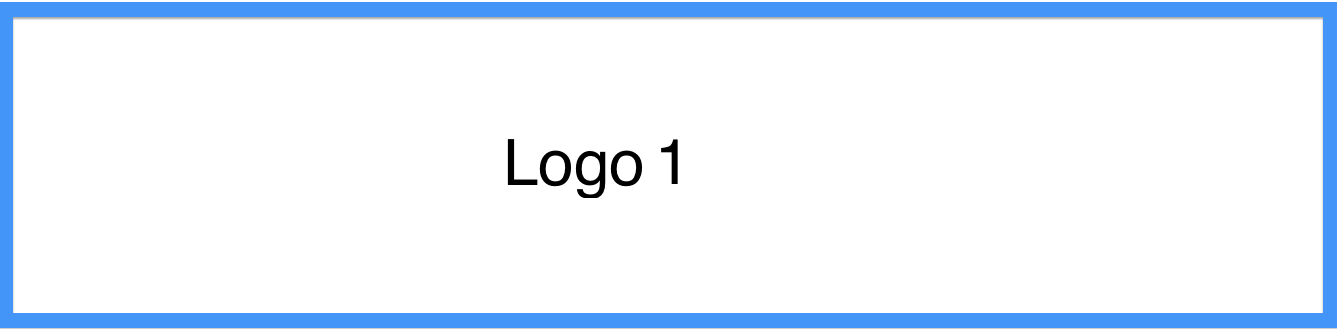
\includegraphics[width=0.4\textwidth,angle=45]{abb/logo1}
 \caption[Beispiel einer Bildbeschreibung]{Beispiel einer Bildbeschreibung\footnotemark}
\label{fig:beispiel1}
\end{figure}
\footnotetext{Bildquelle: Beispielquelle}

% Beispiel für Bildintegration
\begin{figure}[htb]
 \centering
 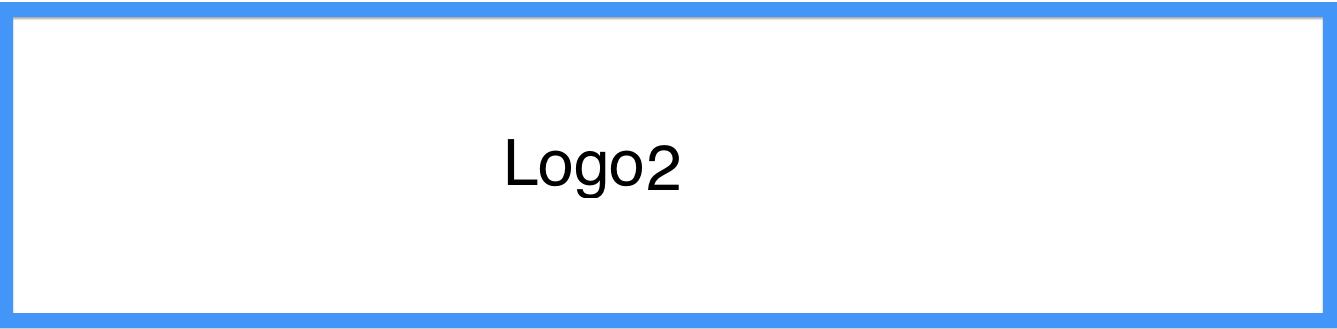
\includegraphics[width=0.3\textwidth,angle=0]{abb/logo2}
 \caption[Beschreibung]{Beschreibung}
\label{fig:Beschreibung}
\end{figure}

% Beispiel: Referenz auf Abbildung
Abbildung~\ref{fig:Beschreibung} [S.\pageref{fig:Beschreibung}]

% Beispiel: Tabelle 
\begin{center}
  \begin{tabular}{ | l | c | }
    \hline
    Überschrift 1 & Überschrift 2 \\ \hline \hline
    Info 1 & Info 2 \\ \hline
    Info 3 & Info 4 \\
    \hline
  \end{tabular}
\end{center}


% Beispiel für Quellcode Listings
\lstset{language=xml}
\begin{lstlisting}[frame=htrbl, caption={Die Datei {\tt data-config.xml} dient als Beispiel für XML Quellcode}, label={lst:dataconfigxml}]
<dataConfig>
  <dataSource type="JdbcDataSource" 
              driver="com.mysql.jdbc.Driver"
              url="jdbc:mysql://localhost/bms_db"
              user="root" 
              password=""/>
  <document>
    <entity name="id"
        query="select id, htmlBody, sentDate, sentFrom, subject, textBody
        from mail">
    <field column="id" name="id"/>
    <field column="htmlBody" name="text"/>
    <field column="sentDate" name="sentDate"/>
    <field column="sentFrom" name="sentFrom"/>
    <field column="subject"  name="subject"/>
    <field column="textBody" name="text"/>
    </entity>
  </document>
</dataConfig>
\end{lstlisting}

\lstset{language=java}
\begin{lstlisting}[frame=htrbl, caption={Das Listing zeigt Java Quellcode}, label={lst:result2}]
/* generate TagCloud */
Cloud cloud = new Cloud();
cloud.setMaxWeight(_maxSizeOfText);
cloud.setMinWeight(_minSizeOfText);
cloud.setTagCase(Case.LOWER);
	    
/* evaluate context and find additional stopwords */
String query = getContextQuery(_context);
List<String> contextStoplist = new ArrayList<String>();
contextStoplist = getStopwordsFromDB(query);
	    
/* append context stoplist */
while(contextStoplist != null && !contextStoplist.isEmpty())
  _stoplist.add(contextStoplist.remove(0));
	    
/* add cloud filters */
if (_stoplist != null) {
  DictionaryFilter df = new DictionaryFilter(_stoplist);
  cloud.addInputFilter(df);
}
/* remove empty tags */
NonNullFilter<Tag> nnf = new NonNullFilter<Tag>();
cloud.addInputFilter(nnf);

/* set minimum tag length */
MinLengthFilter mlf = new MinLengthFilter(_minTagLength);
cloud.addInputFilter(mlf);

/* add taglist to tagcloud */
cloud.addText(_taglist);

/* set number of shown tags */	    
cloud.setMaxTagsToDisplay(_tagsToDisplay);
\end{lstlisting}


% Beispiel für Formeln
Die Zuordnung aller möglichen Werte, welche eine Zufallsvariable annehmen kann nennt man \emph{Verteilungsfunktion} von $X$.

\begin{quotation}
Die Funktion F: $\mathbb{R} \rightarrow$ [0,1] mit $F(t) = P (X \le t)$ heißt Verteilungsfunktion von $X$.\footnote{Konen, vgl.~\cite{wk05}~[S.55]}
\end{quotation}

\begin{quotation}
Für eine stetige Zufallsvariable $X: \Omega \rightarrow \mathbb{R}$ heißt eine integrierbare, nichtnegative reelle Funktion $w: \mathbb{R} \rightarrow \mathbb{R}$ mit $F(x) = P(X \le x) = \int_{-\infty}^{x} w(t)dt$ die \emph{Dichte} oder \emph{Wahrscheinlichkeitsdichte} der Zufallsvariablen $X$.\footnote{Konen, vgl.~\cite{wk05}~[S.56]}
\end{quotation}


\onecolumn
% einfacher Zeilenabstand
\singlespacing
% Literaturliste soll im Inhaltsverzeichnis auftauchen
\newpage
\addcontentsline{toc}{section}{Literaturverzeichnis}
% Literaturverzeichnis anzeigen
\renewcommand\refname{Literaturverzeichnis}
\bibliography{Hauptdatei}

%% Index soll Stichwortverzeichnis heissen
% \newpage
% % Stichwortverzeichnis soll im Inhaltsverzeichnis auftauchen
% \addcontentsline{toc}{section}{Stichwortverzeichnis}
% \renewcommand{\indexname}{Stichwortverzeichnis}
% % Stichwortverzeichnis endgueltig anzeigen
% \printindex

\onehalfspacing
% evtl. Anhang
\newpage
\addcontentsline{toc}{section}{Anhang}
\fancyhead[L]{Anhang} %Kopfzeile links
\subsection*{Anhang}\label{anhang}


% leere Abschlussseite
\newpage
\thispagestyle{empty} % erzeugt Seite ohne Kopf- / Fusszeile
\section*{ }

\end{document}